\chapter{Cronograma de actividades}
\begin{figure}[h]
  \label{figuracronograma1}
  \centering
  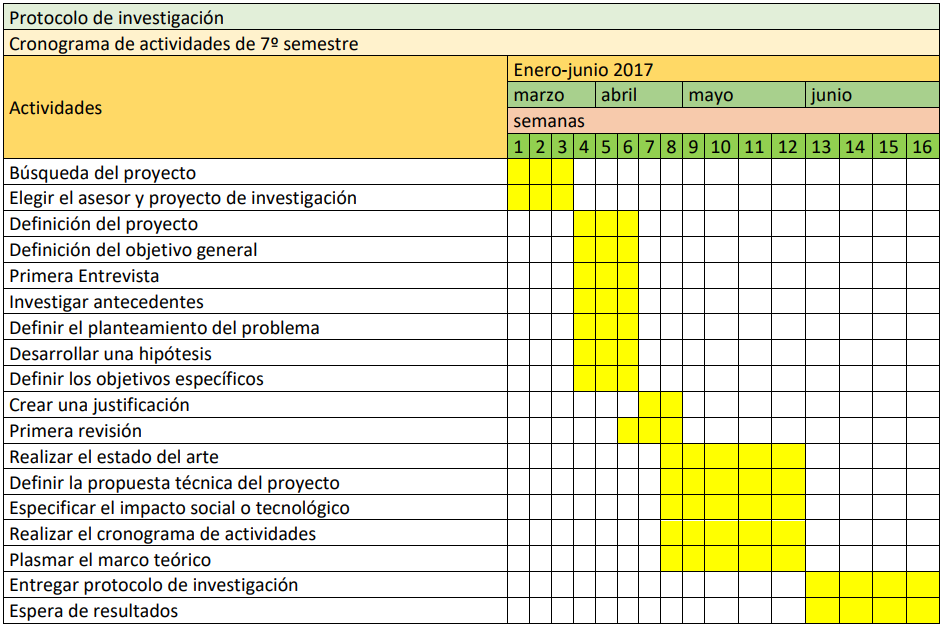
\includegraphics[scale=.5]{lib/assets/cronograma-1}
  \caption{Cronograma de actividades}
\end{figure}

\begin{figure}[h]
  \label{figuracronograma2}
  \centering
  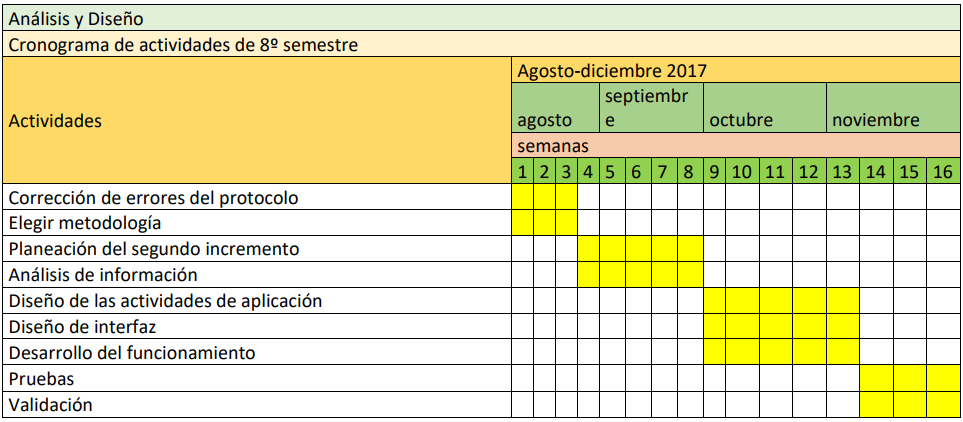
\includegraphics[scale=.5]{lib/assets/cronograma-8-9}
  \caption{Propuesta de cronograma para octavo y noveno semestre}
\end{figure}

\begin{figure}[h]
  \label{figuracronograma3}
  \centering
  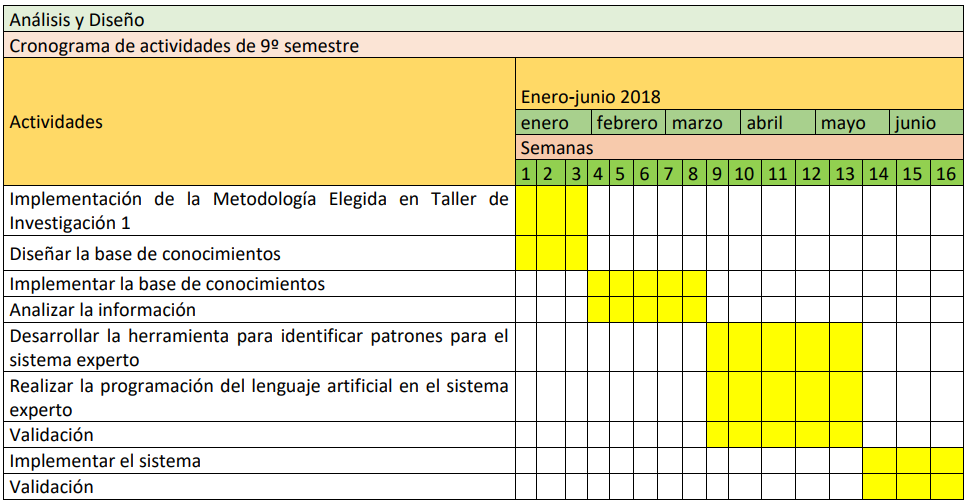
\includegraphics[scale=.5]{lib/assets/cronograma-8-9-2}
  \caption{}
\end{figure}
